\documentclass[dvipdfmx,autodetect-engine]{article}
%---------------------package
\usepackage{geometry}
\usepackage{amssymb}
\usepackage{amsmath}
\usepackage{amsthm}
\usepackage{tikz}
\usetikzlibrary{positioning}

% ----------------------------- 
\theoremstyle{definition}
\newtheorem{Def}{定義}
\newtheorem{Th}{定理}
\newtheorem{Prop}{命題}
\newtheorem{Ex}{例}
\newtheorem{Cor}{系}
\newtheorem{Lem}{補題}
\newtheorem{Prob}{問}

% ------------------------- enumareteで(1)みたいにする
\renewcommand\labelenumi{(\arabic{enumi})}
\renewcommand\labelenumii{(\alph{enumii})}
\renewcommand\labelenumiii{(\roman{enumiii})}

%----------------------------命令定義
\DeclareMathOperator{\Hom}{Hom}
\DeclareMathOperator{\End}{End}
\DeclareMathOperator{\GL}{GL}
\DeclareMathOperator{\gl}{gl}
\DeclareMathOperator{\sllie}{sl}
\DeclareMathOperator{\sublie}{\mathfrak{a}}
\DeclareMathOperator{\lie}{\mathfrak{g}}
\DeclareMathOperator{\cartan}{\mathfrak{h}}
\DeclareMathOperator{\U}{U}


%---------------------------make title
\title{}
\author{}
\date{}
%-----------------------------document
\begin{document}
% \maketitle
    \section{Serreによる包絡環の表示}
    この章では,生成元と関係式から定義されるリー環を定義して,$U(\sllie_n)$の包絡間の表示を求めます.また後半では,$A_{r-1}$型量子群を定義します.
    
    まずは基本的なことの復習から.
    \begin{Def}
        $L := \sllie(n, \mathbb{C}) = \{X \in \gl(n, \mathbb{C}) \mid tr(X) = 0\}$.
        \[
            H := \{ \sum_{i = 1}^{n}x_iE_{ii} \mid \sum_{i = 1}^{n} x_i = 0\}
        \]
        は部分リー環.これをカルタン部分環という.
        また,$L$は$ad(H)$に関する同時固有分解:
        \[
            L = H \oplus (\bigoplus_{i \neq j}\mathbb{C}E_{ij})
        \]
        を持つ($[ad(H), ad(H)] = ad([H,H]) = 0$なので). これをルート分解という.同時固有値は,
        $H$上では$0$,
        $E_ij$上では$x_i - x_j$.
        $x_i - x_j$をルートと呼び,
        $\Delta = \{x_i - x_j\}$
        を$A_{r-1}$型ルート系と呼ぶ.
        また,
        $\alpha_i = x_i - x_{i+1}$
        を単純ルートと呼ぶ.
    \end{Def}
    
    $\sllie_n$に対して次の定理を示すことが前半の目標です.
    \begin{Th}
        \label{main1}
        $L = \sllie(n, \mathbb{C})$の時,$U(L)$は次の生成元と基本関係で定義さ
        れる$\mathbb{C}$上の環$U$と同型.
        
        生成元:
        \[
            e_i, f_i, h_i \quad (1 \leq i \leq n-1)
        \]
        
        基本関係:
        \begin{align}
            e_if_j - f_je_i &= \delta_{ij} h_i\\
            h_ih_j  &= h_jh_i\\
            h_ie_j - e_jh_i &= 
            \begin{cases}
                2e_i \quad (i = j)\\
                -e_j \quad (i - j = \pm 1)\\
                0 \quad (\text{else})
            \end{cases}\\
            h_if_j - f_jh_i &= 
            \begin{cases}
                - 2f_i \quad (i = j)\\
                f_j \quad (i - j = \pm 1)\\
                0 \quad (\text{else})
            \end{cases}\\
            e_i^2e_j - 2e_ie_je_i + e_je_i^2 &= 0 \quad (i - j = \pm 1)\\
            e_ie_j &= e_je_i \quad (\text{else})\\
            f_i^2f_j - 2f_if_jf_i + f_jf_i^2 &= 0 \quad (i - j = \pm 1)\\
            f_if_j &= f_jf_i \quad (\text{else})
        \end{align}
    \end{Th}
    
    \subsection{生成元と基本関係で定義されるリー環}
        生成元と基本関係で定義される結合代数の話のリー環バージョンを話します.これはカッツ・ムーディーリー環との関連で導入されました.
        \begin{Def}
            部分リー環$T(V) \supset L$が$V$で生成される時,これをを$V$で生成される自由リー環と呼び,$L(V)$とかく.$V$の基底を$(X_i)_{i \in I}$とした時には,$L(X \mid i \in I)$などと書くこともある.
        \end{Def}
        
        \begin{Prop}
            自由リー環$L(X_i \mid i \in I)$は普遍写像性質を満たす.
            \[
            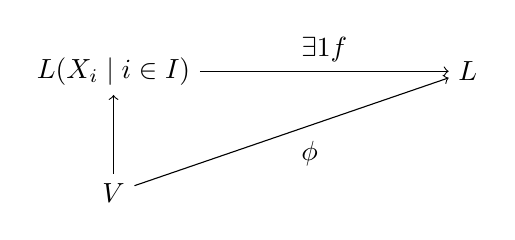
\begin{tikzpicture}[scale = 1.5]
                \node (L) {$L(X_i \mid i \in I)$};
                \node  at (3,0) (EL) {$L$};
                \node[below = of L] (U) {$V$}; 
                
                \draw [->] (L) -- node[above] {$\exists 1 f$}(EL);
                \draw [->] (U) -- node[below left] {} (L);
                \draw [->] (U) -- node[below right] {$\phi$} (EL);
            \end{tikzpicture}
            \]
        \end{Prop}
        \begin{proof}
            $f$は存在すれば一意的.
            実際,hom $f, g: L(X_i \mid i \in I) \to L$が上の可換図式を満たすとすると,
            \[
                f(X_i) = \phi(X_i) = g(X_i)
            \]
            で生成元上の値が一致するので,$f = g$.
            
            次に存在を示そう.
            $\hat{f}:T(V) \to U(L)$を自然な準同型で定める.
            $\epsilon$は包含写像.
            \[
            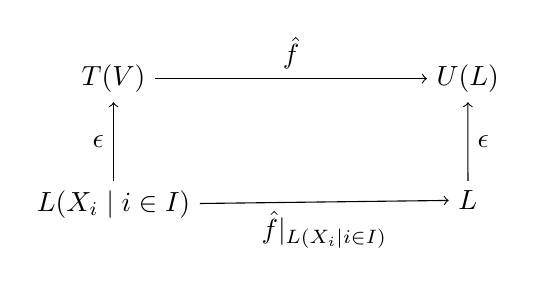
\begin{tikzpicture}[scale = 1.5]
                \node (T) {$T(V)$};
                \node[below = of T] (LX) {$L(X_i \mid i \in I)$}; 
                \node  at (3,0) (U) {$U(L)$};
                \node[below  = of U] (L) {$L$}; 
                
                \draw [->] (T) -- node[above] {$\hat{f}$}(U);
                \draw [->] (L) -- node[right] {$\epsilon$} (U);
                \draw [->] (LX) -- node[left] {$\epsilon$} (T);
                \draw [->] (LX) -- node[below] {$\hat{f}|_{L(X_i \mid i \in I)}$} (L);
            \end{tikzpicture}
            \]  
            すると
            \[
                \hat{f}(L(X_i \mid i \in I)) \subset 
                \hat{L} := \langle\hat{f}(X_i) \mid i \in I \rangle 
                \subset U(L).
            \]
            特に,
            \[
                \hat{f}(L(X_i \mid i \in I)) \subset L
            \]
            よって,$\hat{f}$を制限すれば良い.
        \end{proof}
        特に,リー環$L$の元の族$\{a_i\}_{i \in I}$を取ると,
        \[
            f(X_i) = a_i
        \]
        となるような$f$がただ一つ存在する.
        
        リー環$L$とその元の族$\{a_i\}_{i \in I}$を取る.$F \in L(X_i \mid i \in I)$に対し,
        \[
            F|_{X_i = a_i} := f(F) \in L
        \]
        とする.
        $L(X_i \mid i \in I) \supset \{ F_j \}_{j \in J}$で生成されるイデアル$I = \langle F_i \mid i \in I \rangle$は,
        \[
            \mathcal{I} := \left\{ \sum[H_1, [H_2, [\cdots [H_r, F_j]]]] \right\} \quad(H_i \in L(X_i \mid i \in I), j \in J)
        \]
        という形をしている.
        この時,
        \[
            L(X_i \mid i \in I)/\mathcal{I}
        \]
        を$(X_i)_{i \in I}$を生成元とし,$F_j = 0$を基本関係とするリー環という.
        ここで,$\overline{X_i} = a_i$とかけば,これは$a_i$を生成元とし,$F|_{X_j = a_j}$を基本関係とするリー環ともいう.

        これは次の普遍写像性質で特徴付けられる.
        \begin{Prop}
            $L$を$\{a_i\}_{i \in I}$を生成元とし,$F|_{X_j = a_j}$を基本関係とするリー環とする.
            リー環$H$と,その元の族$\{b_i\}_{i \in I}$が
            \[
                F|_{X_j = b_j} = 0
            \]
            を満たすとする.この時hom $h:L \to H$で$h(a_i) = b_i$を満たすものがただ一つ存在する.
        \end{Prop}
        \begin{proof}
             $h$は生成元で定義されているから,存在すれば一意的なのは明らか.
             自由リー環の普遍性により,
             \[
                f(X_i) = b_i
             \]
             となるhom$f: L(X_i \mid i \in I) \to H$がある.
             この$f$に関して,
             \[
                f(F_j) = 0
             \]
             なので,$f(\langle F_j \rangle) = 0$.
             したがって,
             \[
                h: L(X_i \mid i \in I)/\langle F_j \rangle \to H
             \]
             を誘導し,実際$h(a_i) = b_i$になっている.
        \end{proof}
        
        少し話が逸れるが(前の章に入れるべきだが),生成元と基本関係式で定義される結合代数に関する同様の補題(普遍写像性質)を示しておく.
        \begin{Lem}
            $A$を${a_i}$により生成され,$F_j|_{X_i = a_i}$を基本関係とする結合代数とする.
            結合代数$B$とその元の族${b_i}$があって,$F_j|_{X_i = b_i}$を満たすとする.
            この時,結合代数のhom$h:A \to B$であって$h(a_i) = b_i$を満たすものがただ一つ存在する.
            \[
                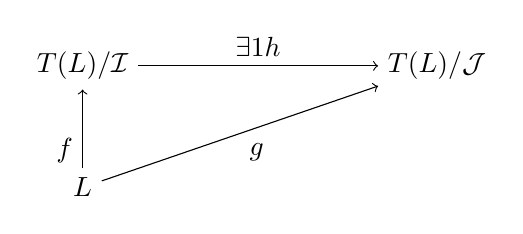
\begin{tikzpicture}[scale = 1.5]
                    \node (A) {$T(L)/\mathcal{I}$};
                    \node  at (3,0) (B) {$T(L)/\mathcal{J}$};
                    \node[below = of A] (L) {$L$}; 
                    
                    \draw [->] (A) -- node[above] {$\exists 1 h$}(B);
                    \draw [->] (L) -- node[below left] {$f$} (A);
                    \draw [->] (L) -- node[below right] {$g$} (B);
                \end{tikzpicture}
            \]
            ここで, $\mathcal{I} \subset \mathcal{J}$.
        \end{Lem}
        \begin{proof}
            $h$があれば,
            \[
                h(F_j|_{X_i = a_i}) = F|_{X_i = b_i}.
            \]
            でなくてはならないから,$h:A \to B$を$h(F_j|_{X_i = a_i}) = F|_{X_i = b_i}$で定めて,これがwell-definedな結合代数の準同型であることを示す.
            $F|_{X_i = b_i}, G|_{X_i = b_i} \in A = T(V)/\mathcal(I)$が
            $F|_{X_i = b_i} = G|_{X_i = b_i}$なら$F - G \in \mathcal{I}$なので,
            \[
                F|_{X_i = b_i} - G|_{X_i = b_i} = (F - G)|_{X_i = b_i} = 0
            \]
            がわかる.したがって$h$は矛盾なく定まる.
            $h$が準同型なのは明らか.
        \end{proof}
        
        
        \begin{Prop}
             $L$を$\{a_i\}_{i \in I}$を生成元とし,$F|_{X_j = a_j}$を基本関係とするリー環とする.
             $F_j \in L(X_i \mid i \in I)$を包含写像で$T(V)$の元とみなそう.このもとで,$\{\overline{a_i}\}_{i \in I}$を生成元とし,$F|_{X_j = \overline{a_i}}$を基本関係とする結合代数を$A$とする.
             この時,
             \[
                U(L) \cong A
             \]
        \end{Prop}
        \begin{proof}
            $A$は$L$と同じ基本関係を満たすから,
            $\exists f: L \to A$で
            \[
                f(a_i) = \overline{a_i}
            \]
            となるリー環のhomがある. 
            $A$が普遍的であることを言えば良い.
            すなわち,
            $B$を結合代数,$g:L \to B$をリー環のhomとする時.
            \[
                h \circ f = g
            \]
            となる結合代数のhom $g:A \to B$がただ一つ存在することを示せばよい.
             \[
                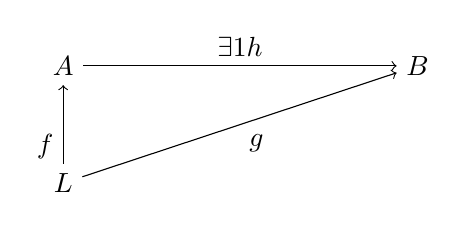
\begin{tikzpicture}[scale = 1.5]
                    \node (A) {$A$};
                    \node  at (3,0) (B) {$B$};
                    \node[below = of A] (L) {$L$}; 
                    
                    \draw [->] (A) -- node[above] {$\exists 1 h$}(B);
                    \draw [->] (L) -- node[below left] {$f$} (A);
                    \draw [->] (L) -- node[below right] {$g$} (B);
                \end{tikzpicture}
            \]
            $h \circ f$と$g$が共にリー環のhomであることはわかっているので,$L$の生成元の上で一致することを確認すれば良い.
            \begin{align*}
                &h \circ f = g\\
                \iff &h(f(a_i)) = g(a_i) \quad (\forall i)\\
                \iff &h(\overline{a_i}) = g(a_i) \quad (\forall i)
            \end{align*}
            $g$はリー環のhomなので,
            \[
                F_j|_{X_i = g(a_i)} = 0
            \]
            が$B$をリー環, $F_j \in L(X_i \mid i \in I)$と思って成り立つ
            ($B$を結合代数,$F_j \in T(V)$でなく)(リー環のhomとしての話なので).
            よって,$F_j|_{X_i = g(a_i)} = 0$は,$B$を結合代数,$F_j \in T(V)$と思っても成り立つ.
            よって,$h(\overline{a_i}) = g(a_i)$を満たす結合代数のhom
            \[
                h: A \to B
            \]
            がただ一つ存在する.
        \end{proof}
        
        ここでようやく本題に戻れる.
        \begin{proof}[Th\ref{main1}'s proof]
            $\sllie_n$が$e_i, f_i, h_i$で生成され,同じ基本関係を満たすリー環であることを示せばよい.
            
            $\sllie_n$の基底として,
            \begin{align}
                h_i &= E_{ii} - E_{i+1, i+1}\\
                e_i &= E_{i,i+1}\\
                f_i &= E_{i+1, i}
            \end{align}
            が取れる.
            これらがTh\ref{main1}の基本関係を満たすことは,行列計算でわかる.
            
            $L$を$E_i, F_i, H_i$を生成元とし,
            Th\ref{main1}の基本関係を$e$を$E$などで置き変えたもの基本関係とするリー環とする.
            $\sllie_n$と$L$の間に同型写像を構成しよう.
            生成元と基本関係で定義された結合代数の普遍性より
            hom $f:L \to \sllie_n$で,
            \[
                f(H_i) = h_i,\, f(E_i) = e_i,\, f(F_i) = f_i
            \]
            となるものがただ一つある.
            この$f$が同型であることを示せば良い.
            生成元が対応しているので,全射は明らか.
            
        \end{proof}
        
    \subsection{$A_{r-1}$型の量子群}
        $\alpha_{j}\left(h_{i}\right) := 2 \delta_{i j}-\delta_{i, j+1}-\delta_{i+1, j}$.
        \begin{Def}
            $K = \mathbb{Q}(q)$を一変数有理函数体とする.
            次の生成元と基本関係で定義される$K$上の単位的結合環を$U_{q}(\sllie_r)$をと書き,$A_{r-1}$型量子群と呼ぶ.
            
            生成元: 
                \[
                    t_i^{\pm1}, e_i, f_i \quad(i = 0, \cdots r-1)
                \]
                
            基本関係:
            \begin{align}
                \begin{array}
                    t_{i} e_{j} t_{i}^{-1}=v^{\alpha_{j}\left(h_{i}\right)} e_{j}, \quad t_{i} f_{j} t_{i}^{-1}=v^{-\alpha_{j}\left(h_{i}\right)} f_{j}\\
                    \left[e_{i}, f_{j}\right]=\delta_{i j} \frac{t_{i}-t_{i}^{-1}}{v-v^{-1}}
                \end{array}\\
                \begin{array}
                    \left[t_{i}, t_{j}\right] = 0, \quad t_{i} t_{i}^{-1} = t_{i}^{-1} t_{i}=1
                \end{array}\\
                \begin{array}
                    {c}{e_{i}^{2} e_{j}-\left(v+v^{-1}\right) e_{i} e_{j} e_{i}+e_{j} e_{i}^{2}=0,(i-j=\pm 1)} \\
                    {e_{i} e_{j}=e_{j} e_{i}(\text{else})}
                \end{array}\\
                \begin{array}
                    {c}{f_{i}^{2} f_{j}-(v+v^{-1}) f_{i} f_{j} f_{i}+f_{j} f_{i}^{2}=0,(i-j=\pm 1)} \\
                    {f_{i} f_{j}=f_{j} f_{i}(\text{else})}
                \end{array}
            \end{align}
        \end{Def}
        最後の4つをSerreの関係式という.
        この環の表現も$L$の表現を変形することで得られる(特に$q = 1$では包絡環と一致する).
        また余積を
        \begin{align*}
            \Delta\left(t_{i}\right)=t_{i} \otimes t_{i}&, \Delta\left(e_{i}\right)=1 \otimes e_{i}+e_{i} \otimes t_{i}^{-1}\\
            \Delta\left(f_{i}\right)&=f_{i} \otimes 1+t_{i} \otimes f_{i}
        \end{align*}
        と変形することでテンソル積表現も作れる.
        \begin{Prop}
            $\Delta: U_q(L) \to U_q(L) \otimes U_q(L)$は環の準同型.
        \end{Prop}
\end{document}
